\documentclass[11pt,a4paper]{article}
\usepackage[spanish]{babel}
\usepackage[utf8]{inputenc}
\usepackage{graphicx}

\usepackage{listings}
\lstset{
language=C,
tabsize=4,
basicstyle=\fontsize{11}{13}\ttfamily\footnotesize,
showspaces=false,
showstringspaces=false,
captionpos=b,
breaklines=true
}

\usepackage{multirow}
\usepackage{float}
\usepackage[caption = false]{subfig}

\begin{document}

%  FRONTPAGE

\begin{titlepage}
  \noindent%
  \begin{tabular}{@{}p{\textwidth}@{}}
    \vspace{0.2cm}
    \begin{center}
    \Huge{\textbf{
      Conjunto de instrucciones MIPS
    }}
    \end{center}
    \begin{center}
      \Large{
         66:20 Organizaci\'on de Computadoras
      }
    \end{center}
    \vspace{0.2cm}\\
  \end{tabular}
  \vspace{4 cm}
  \begin{center}
    {\large
      Trabajo práctico 1
    }\\
    \vspace{0.6cm}
    {\Large
      Axel Lijdens (95772)\\
      Eduardo R Madariaga (90824)\\
      Mauro Toscano (96890)
    }
  \end{center}
  \vfill
  \begin{center}
  Univesidad de Buenos Aires - FIUBA
  \end{center}
\end{titlepage}


\tableofcontents
\pagebreak
% Prologo

\section{Objetivos}

Familiarizarse con el conjunto de instrucciones MIPS32 y el concepto de
ABI, escribiendo un programa portable que trasponga una matriz leida desde un archivo.

\section{Alcance}

Este trabajo práctico es de elaboración grupal, evaluación individual, y de carácter obligatorio para todos alumnos del curso.

\section{Requisitos}

El trabajo deber\'a ser entregado personalmente, en la fecha estipulada, con una car\'atula que contenga los datos completos de todos los integrantes.

Adem\'as, es necesario que el trabajo pr\'actico incluya, la presentaci\'on de los resultados obtenidos, explicando, cuando corresponda, con fundamentos reales, las causas o razones de cada resultado obtenido.

El informe deber\'a respetar el modelo de referencia que se encuentra en el grupo, y se valorar\'an aquellos escritos usando la herramienta TEX / LATEX.

\section{Recursos}

Usaremos el programa GXemul para simular el entorno de desarrollo que utilizaremos en este y otros trabajos prácticos, una máquina MIPS corriendo una versión reciente del sistema operativo NetBSD.
Durante la primera clase del curso presentaremos brevemente los pasos necesarios para la
instalación y configuración del entorno de desarrollo.

\section{Fecha de entrega}

La última fecha de entrega y presentación ser\'a el jueves 26 de abril de 2018.

\section{Informe}\label{informe}
El informe deberá incluir:
\begin{itemize}
\item Documentación relevante al diseño e implementación del programa.
\item Documentación relevante al proceso de compilación: cómo obtener el ejecutable a partir de los archivos fuente.
\item Las corridas de prueba para los archivos matrix1, matrix2, y matrix3.
\item Diagramas del stack de las funciones main y trasponer;
\item El código fuente, en lenguaje C.
\item Este enunciado.
\end{itemize}

% Desarrollo

\section{Implementaci\'on del programa}

Para el dise\~no del programa se empez\'o por establecer los par\'ametros de entrada necesarios:

\begin{itemize}
\item Un archivo de entrada
\item Un archivo de salida opcional. Si ninguno es provisto la salida ser\'a por stdout
\item Opciones para mostrar un mensaje de ajuda y la versi\'on del programa
\end{itemize}

Teniendo en cuenta lo propuesto se escribi\'o el siguiente mensaje de ayuda:

\begin{lstlisting}[numbers=left, tabsize=2, basicstyle=\fontsize{11}{13}\ttfamily, frame=single, caption={Mensaje de ayuda del programa}]
Usage:
   traspuesta -h
   traspuesta -V
   traspuesta [options] filename
Options:
  -h, --help        Prints usage information.
  -V, --version     Prints version information.
  -o, --output      Path to output file.

\end{lstlisting}

Asimismo, se debieron tener en cuenta y validar los siguientes casos en donde alg\'un factor es incorrecto y el mensaje devuelto por el probrama debe ser explicativo del error:

\begin{itemize}
\item \textbf{No se pudo abrir algun archivo:} se debe no solo expresar claramente que se fall\'o al abrir un archivo, sino que tambien se debe especificar si fue en el de entrada o el de salida
\item \textbf{formato inv\'alido del archivo de entrada:} se refiere a una matriz de entrada que no tiene columnas o filas de igual largo, contiene alg\'un caracter especial o no num\'erico, o cualquier divergencia del archivo esperado de entrada.
\item \textbf{Archivos vac\'ios:} solo se aceptar\'an matrices de entrada con al menos una colunma y una fila. 
\end{itemize}

Una vez pasadas las validaciones, se proceder\'a a cargar la matriz primero obteniendo la cantidad de filas/columnas (utilizando estos valores para allocar espacio en memoria que pueda albergar las matrices tanto de entrada como de salida) y luego cargando la matriz de entrada.

Se procede entonces a invocar a la funci\'on trasponer (que se encontrar\'a tanto en assembly como en c\'odigo c), pasandole los siguientes datos:

\begin{itemize}
\item \textit{cantidad\_de\_filas}
\item \textit{cantidad\_de\_columnas}
\item \textit{matriz\_entrada}
\item \textit{matriz\_salida}
\end{itemize}

Finalmente se procede a guardar la matriz obtenida en el archivo de salida (proveido por el usuario o mostrada por stdout) y liberando la memoria que se encuentra alocada para albergar las matrices de entrada y salida.


\section{Compilación del programa}

En el makefile, se especificaron las opciones para compilar el codigo. Es decir, se compilan los archivos \textbf{main.c} y \textbf{matrix.c} en el caso de compilar la totalidad del c\'odigo en c. 

\begin{center}
\textbf{make c}
\end{center}

A la hora de compliar el c\'odigo utilizando la funci\'on escrita en assembly, se utilizaron los archivos \textbf{main.c} y \textbf{matrix.S} con la opci\'on \textbf{-D\_\_MIPS\_\_} para establecer las opciones de compilaci\'on. En este \'ultimo caso se utilizo el entorno propuesto por la c\'atedra para compilar el programa y corer el programa en el sistema operativo NetBSD.

\begin{center}
\textbf{make assembly}
\end{center}

\section{Corridas de prueba}

\begin{figure}
\begin{center}
\subfloat[]{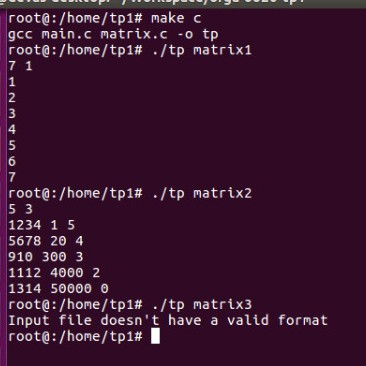
\includegraphics[width=\textwidth,height=\textheight,keepaspectratio]{img/matc.jpeg}} 
\end{center}
\end{figure}

\begin{figure}
\begin{center}
\subfloat[]{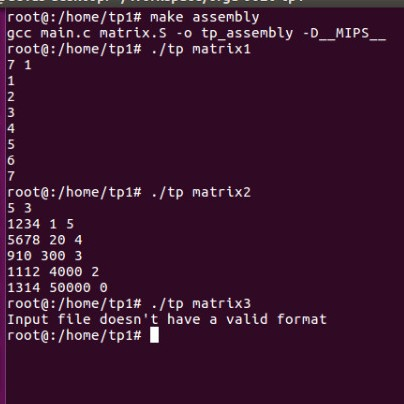
\includegraphics[width=\textwidth,height=\textheight,keepaspectratio]{img/matasm.jpeg}}
\end{center}
\caption{Resultados obtenidos para cada matriz de entrada}
\label{some example}
\end{figure}

Para facilitar el desarrollo se implementó un pequeño conjunto de unit tests de la función trasponer que validan varias entradas y salidas.

Para ejecutar las pruebas basta con utilizar el comando \texttt{make test\_c} o
\texttt{make test\_assembly} y ejecutar el binario resultante. Esto resultó de gran ayuda al momento de desarrollar en assembly ya que permitió verificar rápidamente el correcto funcionamiento de código.

\begin{figure}
\begin{center}
\subfloat[]{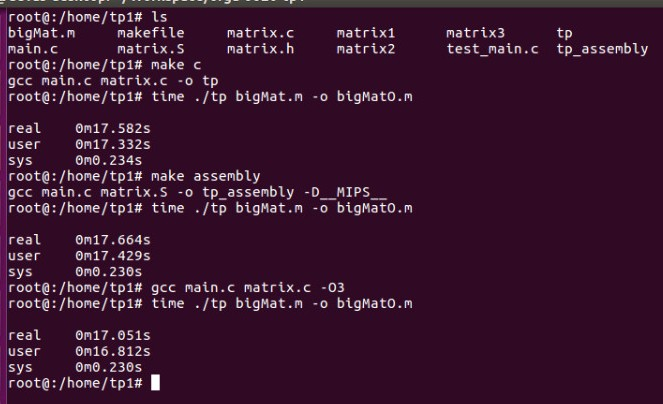
\includegraphics[width=\textwidth,height=\textheight,keepaspectratio]{img/time1.jpeg}}
\end{center}
\end{figure}

\begin{figure}
\begin{center}
\subfloat[]{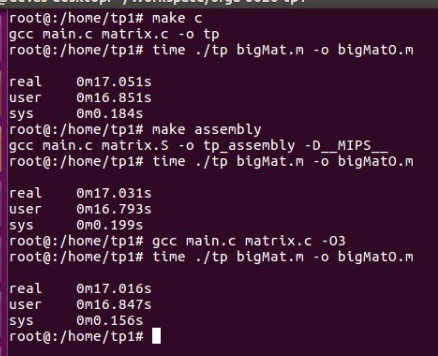
\includegraphics[width=\textwidth,height=\textheight,keepaspectratio]{img/time2.jpeg}}
\end{center}
\end{figure}

\begin{figure}
\begin{center}
\subfloat[]{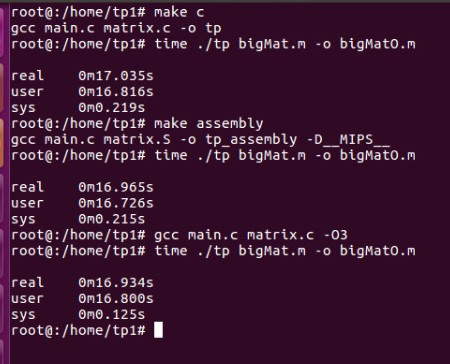
\includegraphics[width=\textwidth,height=\textheight,keepaspectratio]{img/time3.jpeg}} 
\end{center}
\caption{Tiempos de ejecuci\'on para cada matriz de entrada}
\label{some example 2}
\end{figure}

Las salidas para las corridas de las matrices provistas por la c\'atedra se muestran en la figura \ref{some example}. En pantalla se muestran primero las dimensiones de la matriz y luego el contenido de la misma. Notese que para la matriz3, donde el contenido del archivo no es v\'alido, se muestra un mensaje de error apropiado.

Por otro lado, se midieron los tiempos de ejecuci\'on de los programas con la compilaci\'on del metodo \textit{trasponer} en assembly y c, y se obtuvieron resultados pr\'acticamente identicos (difieren en menos del 1\%). Los resultados se muestran en la figura \ref{some example 2}.

Para medir los tiempos se utilizo una matriz que contiene un mill\'on de elementos (cien mil columnas por diez filas), para poder obtener resultados con tiempos apreciables. Nombramos a la matriz \textbf{bigMat.m}, y es la entrada utilizada en las corridas de la Figura \ref{some example 2}.

\section{Diagramas del Stack}

A continuaci\'on se muestra el diagrama de stack utilizado en el desarrollo de
la funci\'on "trasponer":

\begin{table}[h!]
  \begin{center}
    \label{tab:table1}
    \begin{tabular}{|c|c|c}
        \cline{1-2}
        memoria & secci\'on & \\
        \cline{1-2}
        \cline{1-2}
        $a_3$ & \multirow{4}{*}{ABA} & \multirow{4}{*}{caller}\\
        \cline{1-1}
        $a_2$ & &\\
        \cline{1-1}
        $a_1$ & &\\
        \cline{1-1}
        $a_0$ & &\\
        \hline
        $f_p$ & \multirow{2}{*}{SRA} & \multirow{2}{*}{callee}\\
        \cline{1-1}
        $g_p$ & &\\
        \cline{1-2}
    \end{tabular}
    \caption{Stack}
  \end{center}
\end{table}

La funci\'on no tiene ABA propia ya que es hoja. Por la misma raz\'on, no
es necesario guardar el registro $r_a$ ni los registros $s_i$ y la SRA solo necesita tener 8 bytes.
No fue necesario almacenar otros datos en memoria ya que alcanzó con utilizar
los registros $t_i$.

\section{Conclusiones}

Desarrollar una funci\'on en assembly es notablemente mas complicado que su equivalente en C y
adem\'as se pierde la portabilidad provista por el lenguaje. Por otra parte, el compilador
realiza un buen trabajo optimizando el c\'odigo (compilando con -O3) ya que se observ\'o una
leve mejora con respecto a la implementaci\'on en assembly.

Esto indica que no es trivial la optmizaci\'on de esta forma y no siempre
vale la pena, ya que el costo de desarrollo es mucho mayor y por lo tanto, se
debe evaluar bien en que casos se puede lograr una mejora al programar en
assembly, y cu\'al ser\'ia su costo final.

\subsection{Preguntas disparadoras}

\begin{itemize}
\item Se podr\'a hacer mas eficiente el m\'etodo \textit{traspuesta} escrito en assembly?
\item Se podr\'a comparar el codigo asembler que se genera a partir del c\'odigo en c para comparar los pasos y obtener que instrucciones utiliza el compilador en comparaci\'on con las nuestras?
\item Cu\'ales de las instrucciones usadas por el programa son las que consumen la mayor parte del tiempo?
\end{itemize}

\subsection{Problemas encontrados a lo largo del proyecto}

Es f\'acil introducir bugs sutiles en el programa que luego son dificiles de 
encontrar. Durante el desarrollo se debi\'o utilizar GDB, pero fue importante
investigar sobre su uso, ya que se deben usar las directivas "stepi" o "nexti"
para poder avanzar instrucciones individuales.

\subsection{Futuras investigaciones}

Respecto a los temas tratados en el presente proyecto, se podr\'ia estudiar que cambios se pueden hacer sobre la implementaci\'on en assembly para lograr que sea m\'as eficiente que c compilado con -O3. Asimismo, se podr\'ia hacer un an\'alisis de las instrucciones usadas por el compilador a la hora de compilar el programa.

% SOlO codigos fuente hacia abajo, no hace falta editar!

\newpage

\section{C\'odigos fuente}

Repositorio: https://github.com/voices117/orga-6620-tp1

\subsection{MakeFile}

\begin{lstlisting}[numbers=left, tabsize=2, basicstyle=\fontsize{11}{13}\ttfamily, frame=single, caption={makefile}]
GCC_FLAGS = -std=c99

c: main.c matrix.c
	gcc $(GCC_FLAGS) main.c matrix.c -o tp

assembly: main.c matrix.S
	gcc $(GCC_FLAGS) main.c matrix.S -o tp_assembly -D__MIPS__

test_c: test_main.c matrix.c
	gcc $(GCC_FLAGS) test_main.c matrix.c -o test_c

test_assembly: test_main.c matrix.S
	gcc $(GCC_FLAGS) test_main.c matrix.S -o test_assembly -D__MIPS__

\end{lstlisting}

\subsection{Main}

\begin{lstlisting}[numbers=left, tabsize=2, basicstyle=\fontsize{11}{13}\ttfamily, frame=single, caption={makefile}]
#include <ctype.h>
#include <getopt.h>
#include <inttypes.h>
#include <stdbool.h>
#include <stddef.h>
#include <stdint.h>
#include <stdio.h>
#include <stdlib.h>
#include <unistd.h>
#include <string.h>
#include "matrix.h"

struct args {

  /* Path del archivo con los datos de entrada */
  const char* path_entrada;

  /* Path salida */
  const char* path_salida;
  
  /* Boolean indica si se usa stdout */
  bool usa_std_out;
};


/** Estructura que uitliza getopt_log para parsear los argumentos de linea de
 * comandos. */
static const struct option _long_opts[] = {
    {.name = "help", .has_arg = no_argument, .flag = NULL, .val = 'h'},
    {.name = "version", .has_arg = no_argument, .flag = NULL, .val = 'V'},
    {.name = "output", .has_arg = required_argument, .flag = NULL, .val = 'o'},
    {0},
};

/**
 * @brief Imprime un mensaje de ayuda y termina el programa.
 *
 * @param bin_name argv[0].
 */
static void _print_help(const char *bin_name) {
  printf("Usage:\n");
  printf("   traspuesta -h\n");
  printf("   traspuesta -V\n");
  printf("   traspuesta [options] filename\n");
  printf("Options:\n");
  printf("  -h, --help        Prints usage information.\n");
  printf("  -V, --version     Prints version information.\n");
  printf("  -o, --output      Path to output file.\n");
}

/**
 * @brief Imprime la version del programa y termina.
 *
 * @param bin_name argv[0].
 */
static void _print_version(const char *bin_name) {
  printf("%s, version 1.00\n", bin_name);
}

static void _arg_parse(struct args* args,int argc, const char **argv) {
    
  int ch = -1;
  args->usa_std_out = true;

  while ((ch = getopt_long(argc, (char **)argv, "hVo:", _long_opts, NULL)) != -1) {
    switch (ch) {
      case 'h':
        _print_help(argv[0]);
        exit(0);
        break;

      case 'V':
        _print_version(argv[0]);
        exit(0);
        break;
        
      case 'o':
        args->usa_std_out = false;
        args->path_salida = argv[optind - 1];
        break;
        
      /* this is returned when a required argument was not provided */
      case '?':
        exit(1);
        break;
      
    }
  }
  
  if(optind < argc){
    args->path_entrada = argv[optind]; 
    optind++;       
    }else{ 
       fprintf( stderr, "No file specified\n"); 
       exit(1); 
    }
}

void abrir_archivos(struct args args, FILE** archivo_entrada, FILE** archivo_salida){
    *archivo_entrada = fopen(args.path_entrada, "r");
    if (*archivo_entrada == 0) {
       perror("Input file error");
    }
    
    if(args.usa_std_out)
        *archivo_salida = stdout;
    else{
        *archivo_salida = fopen(args.path_salida, "w");
        if (*archivo_salida == 0) {
            perror("Output file error");
        }
    }
    
    //Si alguno de los dos fallo cancelo lo hecho y salgo
    if(*archivo_entrada == 0 || *archivo_salida == 0){
        
        if(*archivo_entrada != 0){
            fclose(*archivo_entrada);
        }
        
        if(*archivo_salida != 0){
            fclose(*archivo_salida);
            remove(args.path_salida);
        }
        
        exit(1);
    }
}

int main(int argc, const char *argv[]){
    struct args args;
    FILE* archivo_entrada;
    FILE* archivo_salida;
    int cantidad_de_filas;
    int cantidad_de_columnas;
    int cantidad_de_filas_traspuesta;
    int cantidad_de_columnas_traspuesta;
    long long int* matriz_entrada;
    long long int* matriz_salida;
    int indice_matriz_entrada = 0;
    char* direccion_caracter_no_numerico = NULL;
    char string_cargado[50];
    long long int numero_cargado;
    _arg_parse(&args,argc, argv);
    
    abrir_archivos(args, &archivo_entrada, &archivo_salida);

    fscanf(archivo_entrada, "%s ", string_cargado);
    cantidad_de_filas = strtol(string_cargado, &direccion_caracter_no_numerico, 0);
    if(*direccion_caracter_no_numerico != '\0'){
        fprintf( stderr, "Input file doesn't have a valid format\n"); 
        exit(1);
    }
    if(cantidad_de_filas < 1){
        fprintf( stderr, "Number of rows must be positive\n"); 
        exit(1);
    }
        
        
    fscanf(archivo_entrada, "%s ", string_cargado);
    cantidad_de_columnas = strtol(string_cargado, &direccion_caracter_no_numerico, 0);
    if(*direccion_caracter_no_numerico != '\0'){
        fprintf( stderr, "Input file doesn't have a valid format\n"); 
        exit(1);
    }
    if(cantidad_de_columnas < 1){
        fprintf( stderr, "Number of columns must be positive\n"); 
        exit(1);
    }
    
    matriz_entrada = malloc(sizeof(long long int) * cantidad_de_filas * cantidad_de_columnas);
    matriz_salida = malloc(sizeof(long long int) * cantidad_de_filas * cantidad_de_columnas);
    
    //Cargo la matriz de entrada
    while(fscanf(archivo_entrada, "%s ", string_cargado) != EOF){
        
        numero_cargado = strtoll(string_cargado, &direccion_caracter_no_numerico, 0); //Esta en base 10;
        
        if(*direccion_caracter_no_numerico != '\0'){
            fprintf( stderr, "Input file doesn't have a valid format\n"); 
            exit(1);
        }
        
        matriz_entrada[indice_matriz_entrada] = numero_cargado;
        indice_matriz_entrada++;
        
    }
    
    trasponer(cantidad_de_filas, cantidad_de_columnas, matriz_entrada, matriz_salida);
    cantidad_de_columnas_traspuesta = cantidad_de_filas;
    cantidad_de_filas_traspuesta = cantidad_de_columnas;
    
    fprintf(archivo_salida, "%u %u\n", cantidad_de_filas_traspuesta, cantidad_de_columnas_traspuesta );
    
    unsigned i,j;
    for (i = 0; i < cantidad_de_filas_traspuesta; i++) {
        for (j = 0; j < cantidad_de_columnas_traspuesta; j++) {
            fprintf(archivo_salida, "%lld ",matriz_salida[i * cantidad_de_columnas_traspuesta + j]);
        } 
        fputc('\n', archivo_salida);
    }
    
    free(matriz_entrada);
    free(matriz_salida);
    
}

\end{lstlisting}


\subsection{Matrix Method (c)}

\begin{lstlisting}[numbers=left, tabsize=2, basicstyle=\fontsize{11}{13}\ttfamily, frame=single, caption={Matrix method (c)}]
#include "matrix.h"

/**
 * @brief Transpone una matriz almacenada en un array de long long.
 *
 * @param filas Cantidad de filas en la matriz.
 * @param columnas Cantidad de columnas en la matriz.
 * @param entrada Puntero a la matriz de entrada.
 * @param salida Puntero a la matriz de salida.
 * @return 0 siempre.
 */
int trasponer(unsigned int filas, unsigned int columnas, const long long *entrada,
              long long *salida) {
  unsigned i,j;
  for (i = 0; i < filas; i++) {
    for (j = 0; j < columnas; j++) {
      salida[j * filas + i] = entrada[i * columnas + j];
    }
  }

  return 0;
}
\end{lstlisting}


\subsection{Matrix.h}

\begin{lstlisting}[numbers=left, tabsize=2, basicstyle=\fontsize{11}{13}\ttfamily, frame=single, caption={Matrix method (c)}]
#ifndef MATRIX_H
#define MATRIX_H

/** Transpone una matriz. */
int trasponer(unsigned int filas, unsigned int columnas, const long long *entrada,
              long long *salida);

#endif
\end{lstlisting}


\subsection{Matrix Method (asm)}

\begin{lstlisting}[numbers=left, tabsize=2, basicstyle=\fontsize{11}{13}\ttfamily, frame=single, caption={matrix method (asm}]
#include <mips/regdef.h>

# trasponer(unsigned int, unsigned int, long long const*, long long*):
.global trasponer
trasponer:
    subu    sp, sp, 8       # muevo el stack pointer
    sw      $fp, 4(sp)
    sw      gp, 0(sp)

    # parametros de entrada
    sw        a0, 8(sp)      # filas
    sw        a1, 12(sp)     # columnas
    sw        a2, 16(sp)     # entrada
    sw        a3, 20(sp)     # salida

    # inicializa las variables locales
    li        t0, 0          # $t0 = 0 (contador filas)
    li        t2, 0          # $t2 = 0 (condicion de corte loop filas)

loop_rows:
    slt     t2, t0, a0       # if( a0 <= t0 )
    beq      t2, zero, end   #   goto end;

    # inicializa el loop de columnas
    li        t1, 0          # $t1 = 0 (contador columnas)
    li        t3, 0          # $t3 = 0 (condicion de corte loop columnas)

loop_cols:
    slt     t3, t1, a1          # if( a1 <= t1 )
    beq     t3, zero, end_cols  #   goto end_cols;

    # copia el valor de la matriz de entrada a la de salida
    mulou   t4, t1, a0        # t4 = t1 * a0 + t0 (indice de salida)
    addu    t4, t0
    sll     t4, t4, 3         # multiplica por 8
    addu    t4, a3

    mulou   t5, t0, a1        # t5 = t0 * a1 + t1 (indice de entrada)
    addu    t5, t1
    sll     t5, t5, 3
    addu    t5, a2

    lw      t6, 0(t5)         # carga el valor del indice
    lw      t7, 4(t5)         # en 2 partes (por ser un long long)

    sw        t6, 0(t4)       # copia las 2 words
    sw        t7, 4(t4)       # copia las 2 words

    # incrementa el contador de columas
    addi    t1, t1, 1         # t1 = t1 + 1
    j        loop_cols        # jump a loop_cols

end_cols:
    # incrementa el contador de filas
    addi    t0, t0, 1         # t0 = t0 + 1
    j        loop_rows        # jump a loop_cols

end:
    # restaura los resgitros
    lw        gp, 0(sp)
    lw        $fp, 4(sp)
    li        v0, 0         # v0 = 0
    addiu     sp, sp, 8     # libera el stack
    jr        ra            # retorna


\end{lstlisting}

\end{document}